%%%%%%%%%%%%%%%%%%%%%%%%%%%%%%%%%%%%%%%%%%%%%%%%%%%%%%%%%%%%%%%%%%%%%%%%%%%%%%
% University of Bristol presentation theme based on the PowerPoint template
%
% Copyright (c) 2012, 2020 David A.W. Barton (david.barton@bristol.ac.uk)
% All rights reserved.
%
% The latest version of this theme can be found at
%   https://github.com/db9052/UoB-beamer-theme
% 

\documentclass[aspectratio=169]{beamer}
    % Possible aspect ratios are 16:9, 16:10, 14:9, 5:4, 4:3 (default) and 3:2
    % (Remember to remove the colon, i.e., 16:9 becomes the option 169)
    \usepackage{soul}


\usetheme{UoB}


\sethlcolor{BrightBlue}

\title[Quantum Scrambling]{Scrambling Encoded Information}
\subtitle{Physics Research Project}
\author{Samuel A. Hopkins}
\institute{Theoretical Physics MSci}
\date{23rd March 2023}

%%%%%%%%%%%%%%%%%%%%%%%%%%%%%%%%%%%%%%%%%%%%%%%%%%%%%%%
% Start of the slides

\begin{document}
\urltext{}
\logo{logo}
% [leftcolor=CoolGrey,rightcolor=BrightPurple,div=0.8\paperwidth]
% Available frame options:
%   leftcolor, rightcolor: set the colour of the left or right panel
%   leftimage, rightimage: put a (cropped) image in the left or right panel
%   div: set the location of the divider between left and right panels
%   urlcolor: set the colour of the url

% Other commands available:
%   \logo{X}: choose the logo to display (logo, white logo, or black logo)
%   \urltext{X}: change the url for each slide

% All standard University of Bristol colours are available:
%   UniversityRed, CoolGrey, BrightAqua, BrightBlue, BrightOrange, BrightPurple,
%   BrightPink, BrightLime, DarkAqua, DarkBlue, DarkOrange, DarkPurple,
%   DarkPink, DarkLime

\begin{frame}
  \titlepage
\end{frame}

%%%%%%%%%%%%%%%%%%%%%%%%%%%%%%%%%%%%%%%%%%%%%%%%%%%%%%%%%%%%%%%%%%%%%%%%%%%%%%
\lecture{Lecture 1}{01}

%Presentation Plan
%Introduction to quantum scrambling
%operator spreading + entanglement Entropy
%Look at the two quantum circuit models, leave maths out -motivate the need
%Results and the conclusions drawn from it

\input{QS_Subfiles/QS_introduction.tex}
% \begin{frame}{Simulating Spin Systems}
% Quantum Systems are BIG. scaling is typically ${\cal{O}}(2^N)$ in system size, $N$. Can only simulate 10-15 qubits. 

% To simulate unitary evolution, quantum circuits are ideal, there are 3 classes of quantum circuits that can be simulated in polynomial time. 
% \begin{itemize}
%     \item Stabilizer or Clifford circuits
%     \item Non-interacting Fermion circuits
%     \item Dual-Unitary Circuits
% \end{itemize}
% We focus on the first two. To showcase quantum scrambling, we need a system that becomes highly entangled from an initially local operator (to show operator spreading)
% \end{frame}

\begin{frame}{Clifford Circuits}
    Circuits comprised of gates from the Clifford Group: $\{H, CNOT, S\}$
    %Built upon work by Blake and Linden (ref)

    \begin{itemize}
        \item Not sufficient to generate operator complexity: $H X H^{\dagger} = Z$
        \item Can recover operator complexity with a non-local description of Pauli strings \cite{Blake_2020}.
        \item This sacrifices any notion of operator spreading. Initial operator has support over the entire system.
    \end{itemize}

    \begin{columns}
        \begin{column}{0.475\textwidth}
            \begin{figure}
            \vspace{-3cm}
            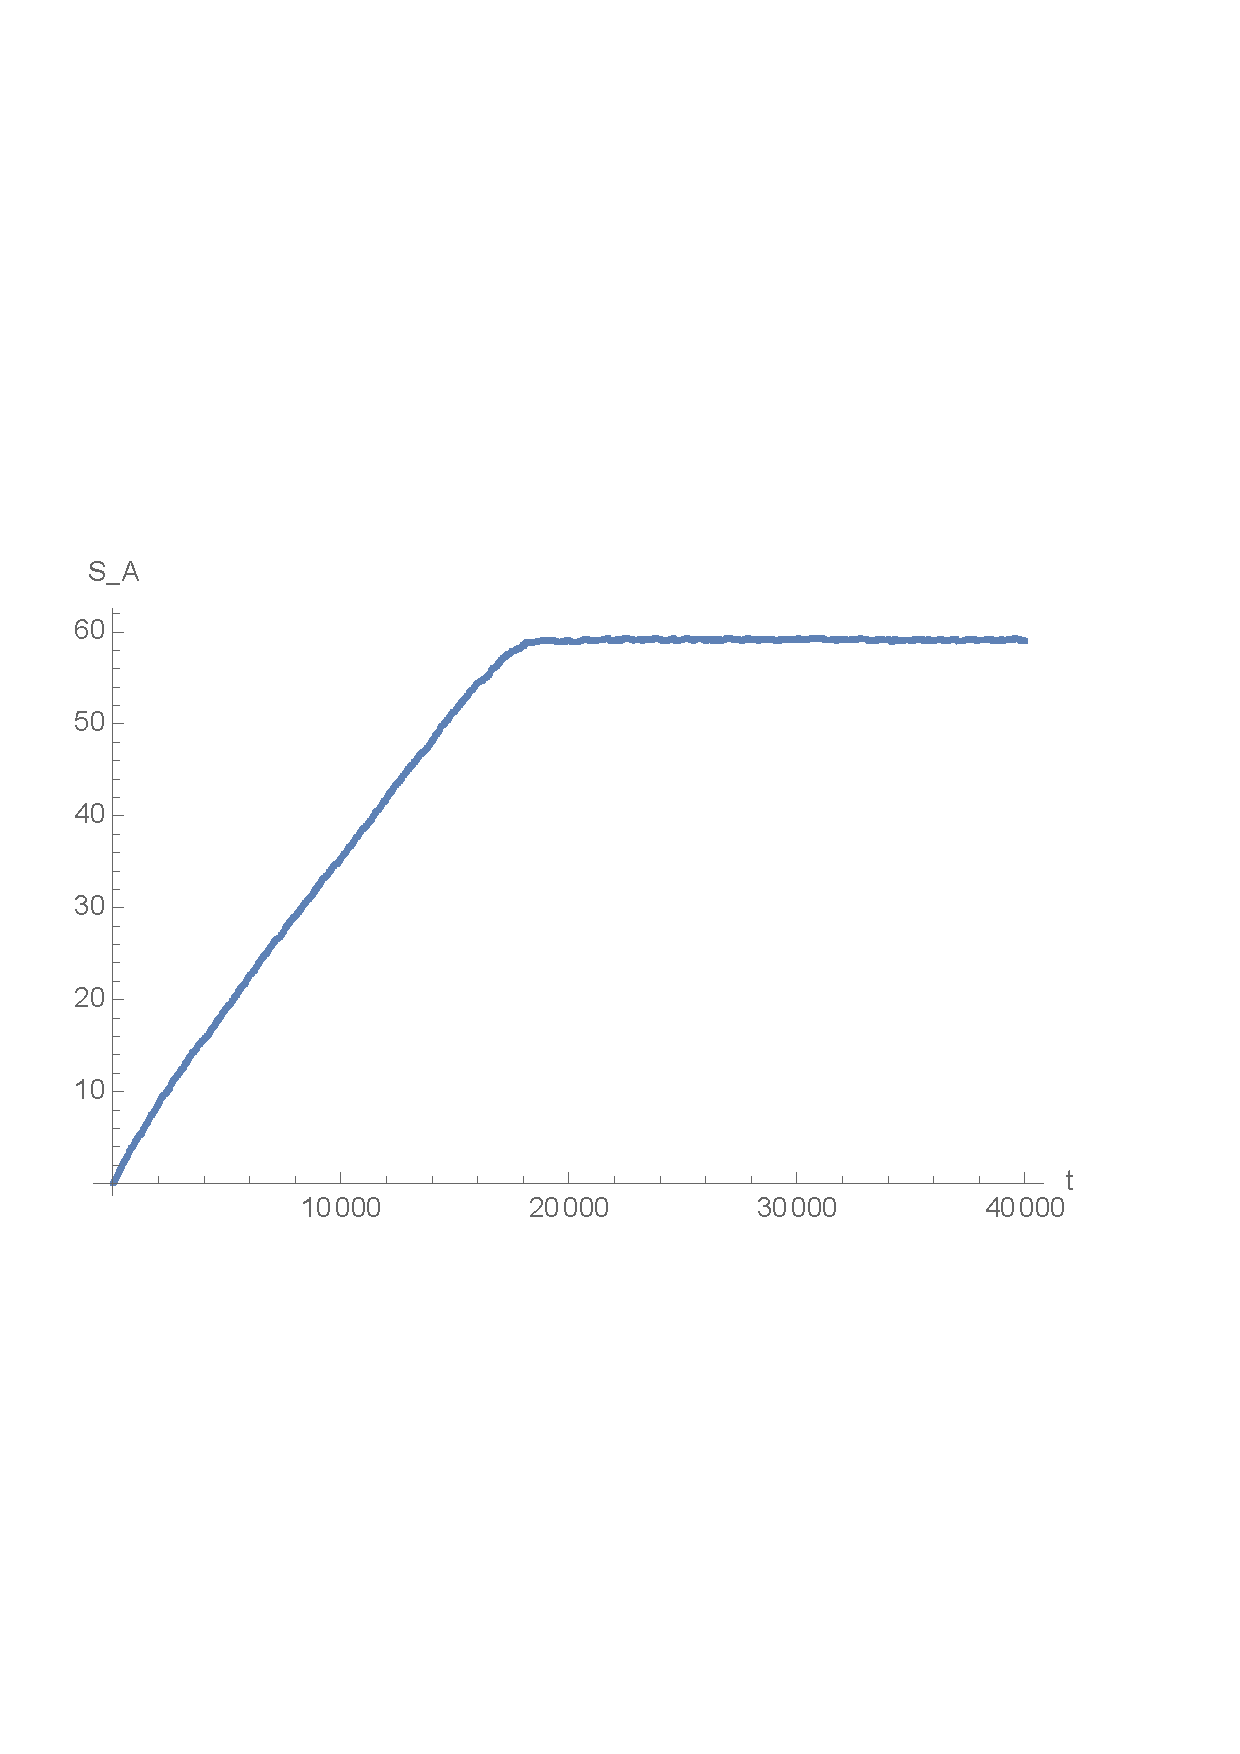
\includegraphics[width = \textwidth]{QS_Images/BAL_Result.pdf}
        \end{figure}
        \end{column}

        \begin{column}{0.475\textwidth}
            \begin{figure}
                \vspace{-3cm}
                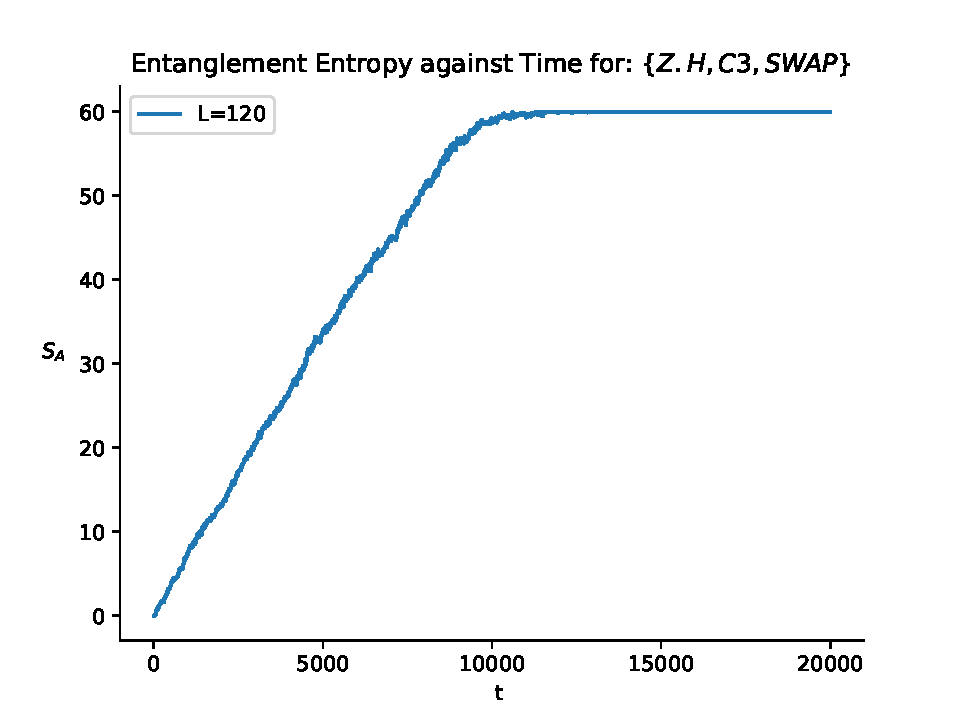
\includegraphics[width = \textwidth]{QS_Images/BAL_reconstruction.pdf}
            \end{figure}
        \end{column}

    \end{columns}

    %Show Blake and linden picture, Then state we tried to do somethiing similar for a local operator. However it doesnt work since any operator gets mapped to another product of pauli's. 
\end{frame}

\begin{frame}{Fermionic Systems}
    %instead of using qubits and pauli operators, we can use fermionic operators to describe circuits
    We can describe quantum circuits using operators from second quantization, namely the creation, $a_i^{\dagger}$ and annihilation, $a_i$ operators.

    \begin{itemize}
        \item System of $N$ qubits: $|n_1\rangle \otimes |n_2\rangle \otimes \dots \otimes |n_L\rangle$
        \item System of $N$ Local Fermionic Modes: $|n_1, n_2, \dots, n_L \rangle \equiv (a_1^{\dagger})^{n_1}(a_2^{\dagger})^{n_2} \dots (a_L^{\dagger})^{n_L} |\underline{\bf{0}}\rangle$.
    \end{itemize}





    Obey crucial anti-commutation relations:
    \begin{align*}
        \{a_i, a_j\} = \{a_i^{\dagger}, a_j^{\dagger}\} \equiv 0 && \{a_i, a^{\dagger}_j\} = \delta_{ij} I
    \end{align*}
    To enforce anti-commutation relations, fermionic operators are defined using global operators. Implies inherent non-locality to fermionic description.
    
    %insert image to show hopping hamiltonian.
 
\end{frame}
\begin{frame}{Non-interacting Fermion Circuits}


    \begin{columns}
        \begin{column}{0.475\textwidth}
 
    \begin{itemize}
        \item Use fermionic operators to construct unitary gates: $U = \exp(i\frac{\pi}{4} (a^{\dagger}_{0} a_{1} + a^{\dagger}_{1}a_{0}))$ 
        \item Build a circuit using unitary gates. For non-interacting Fermions, no terms higher than quadratic order in fermionic operators.
        \item Shown to be classically simulable by Terhal and DiVincenzo \cite{Terhal_2002}.
        \item  Also has been shown to exhibit Operator Spreading and a growth in entanglement entropy. Good candidate for studying quantum scrambling.
    \end{itemize}

\end{column}
\begin{column}{0.475\textwidth}
    \begin{figure}
        \vspace{-3cm}
        \centering
        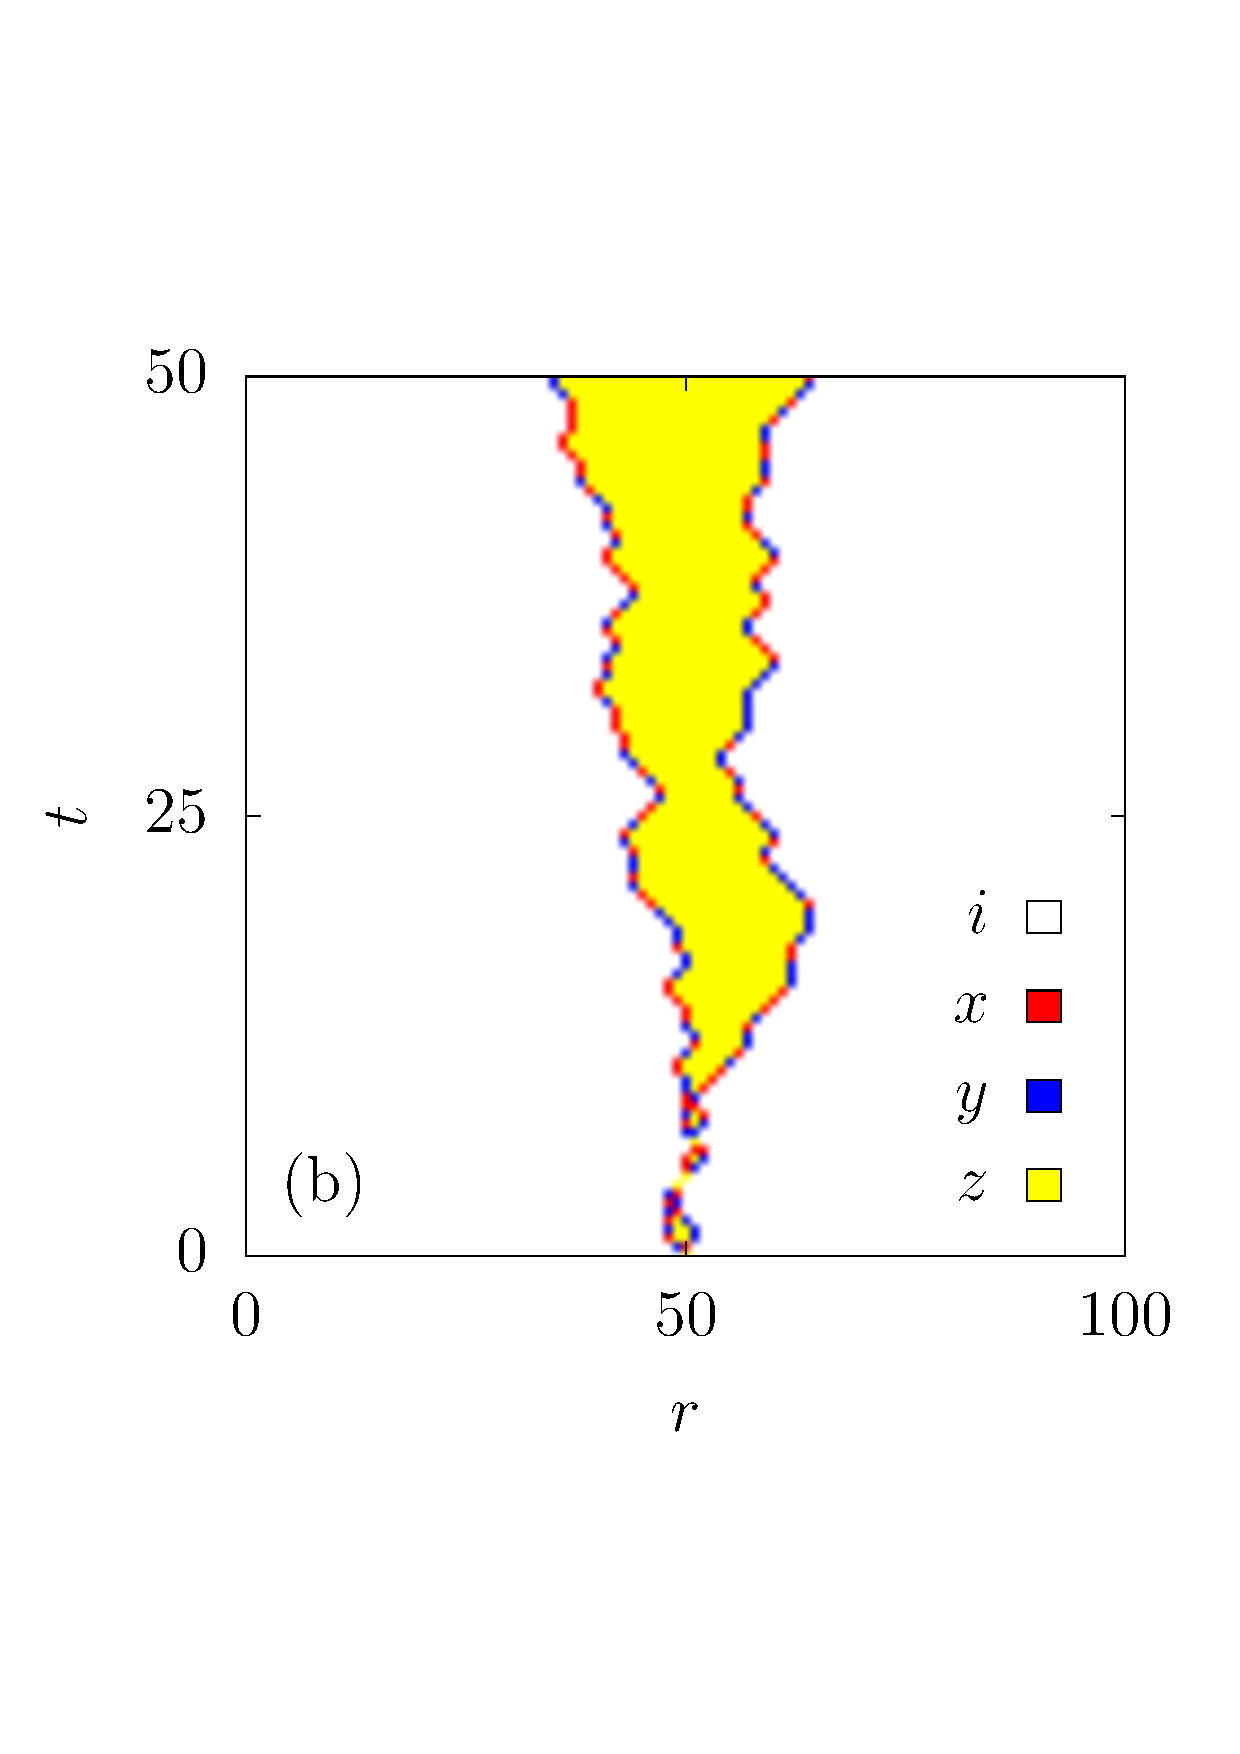
\includegraphics[width = 0.8\textwidth]{QS_Images/freefermionspread.pdf}
        \vspace{-1.5cm}
        \caption{Operator spreading in Free Fermion Circuit \cite{dias2021diffusive}}
    \end{figure}
\end{column}
    % \begin{figure}
    %     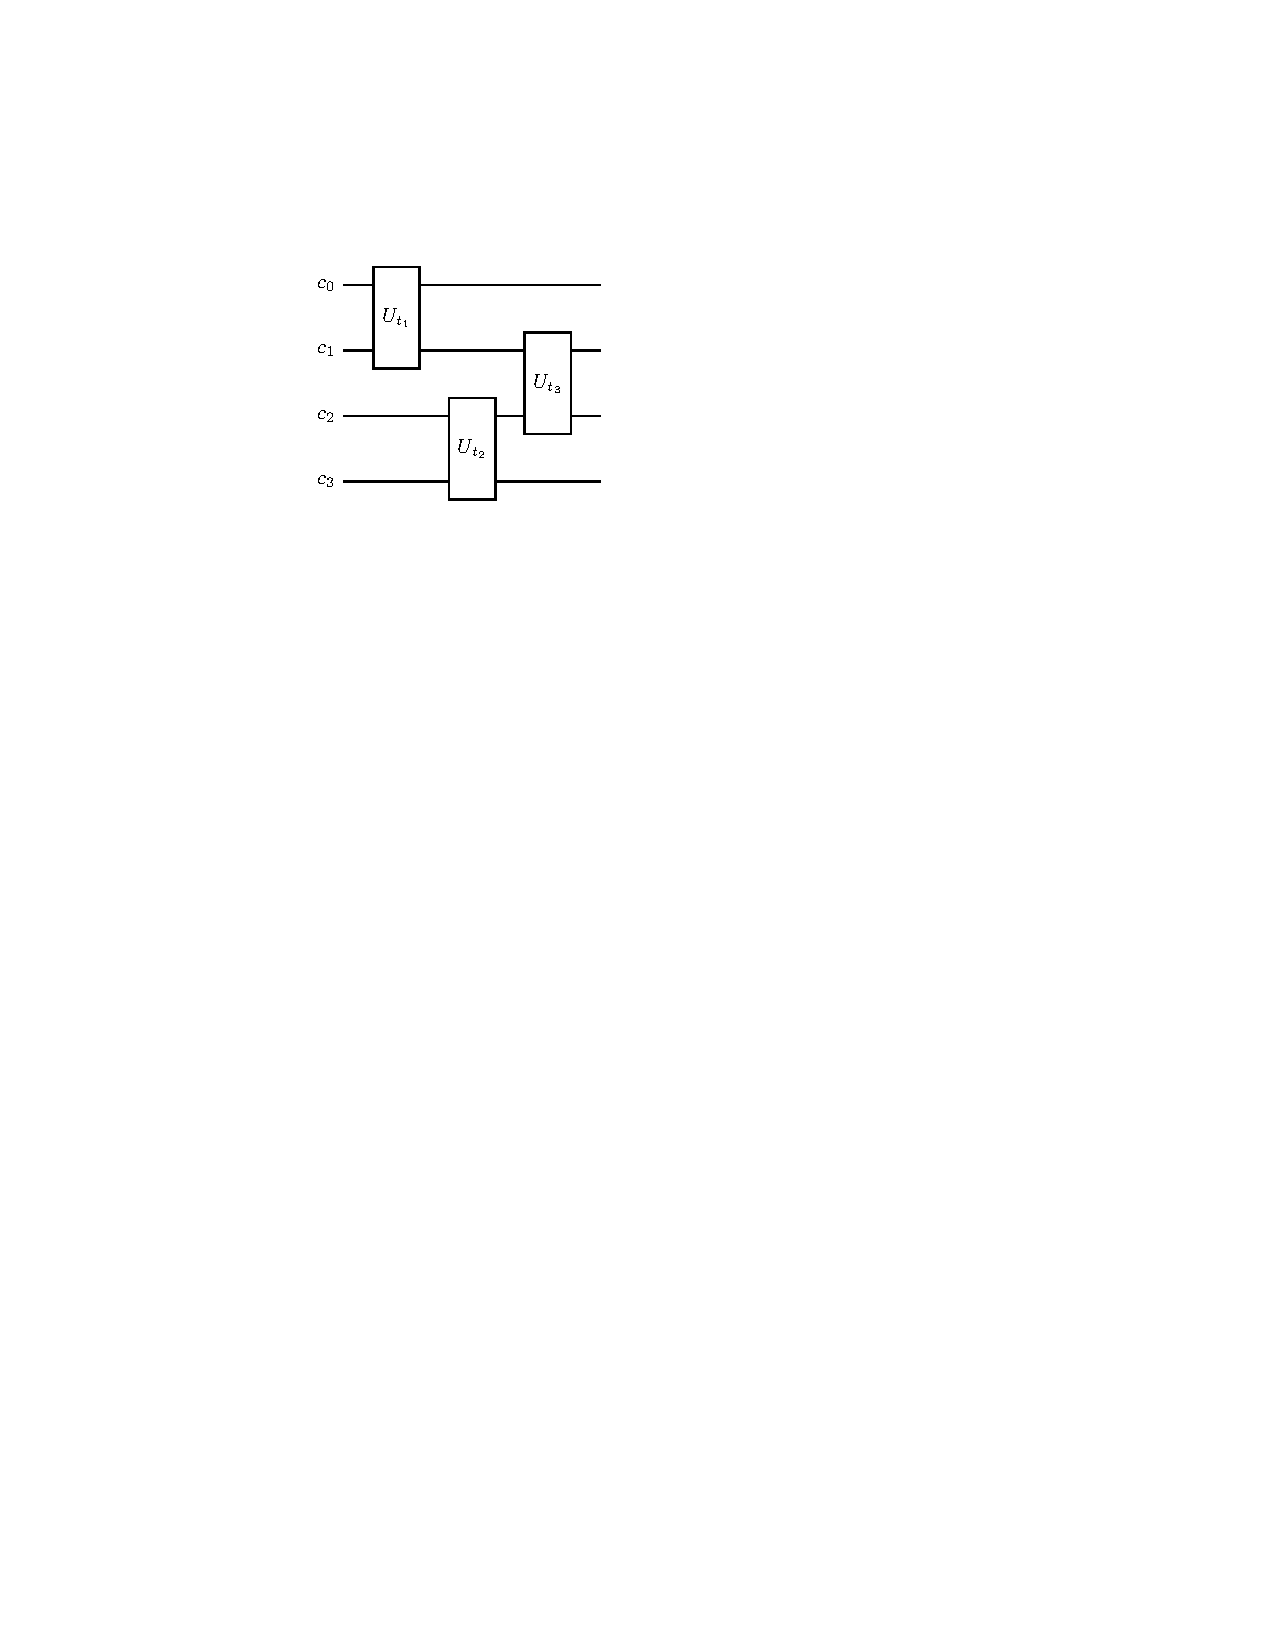
\includegraphics{QS_Images/quantikz (1).pdf}
    % \end{figure}
   

\end{columns}
\end{frame}

    \begin{frame}{Non-Interacting Fermion Circuits - Results}
\begin{columns}
    \begin{column}{0.475\textwidth}
        \begin{figure}
            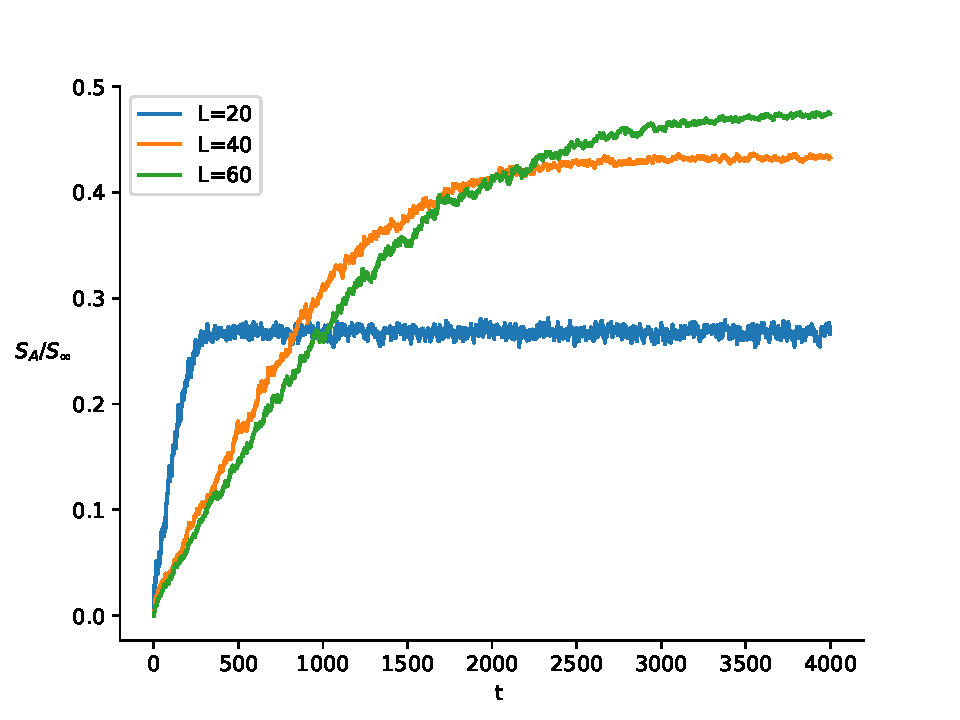
\includegraphics[width = \textwidth]{QS_Images/EntanglementEntropy_varL.pdf}
            \caption{Numerical results for a free fermion circuit with system size, $L=$20, 40, and 60.}
        \end{figure}
    \end{column}

    \begin{column}{0.5\textwidth}
        \begin{itemize}
            \item Free fermion circuits exhibit quantum scrambling.
            \item Free Fermion circuits weakly scramble.
            \item Smaller system sizes saturate earlier. 
            \item Entropy saturation value is dependent on system size.
        \end{itemize}
    \end{column}




\end{columns}
        
    \end{frame}


    \begin{frame}{Comparison}
        \begin{columns}
            \begin{column}{0.475\textwidth}
                \begin{figure}
                    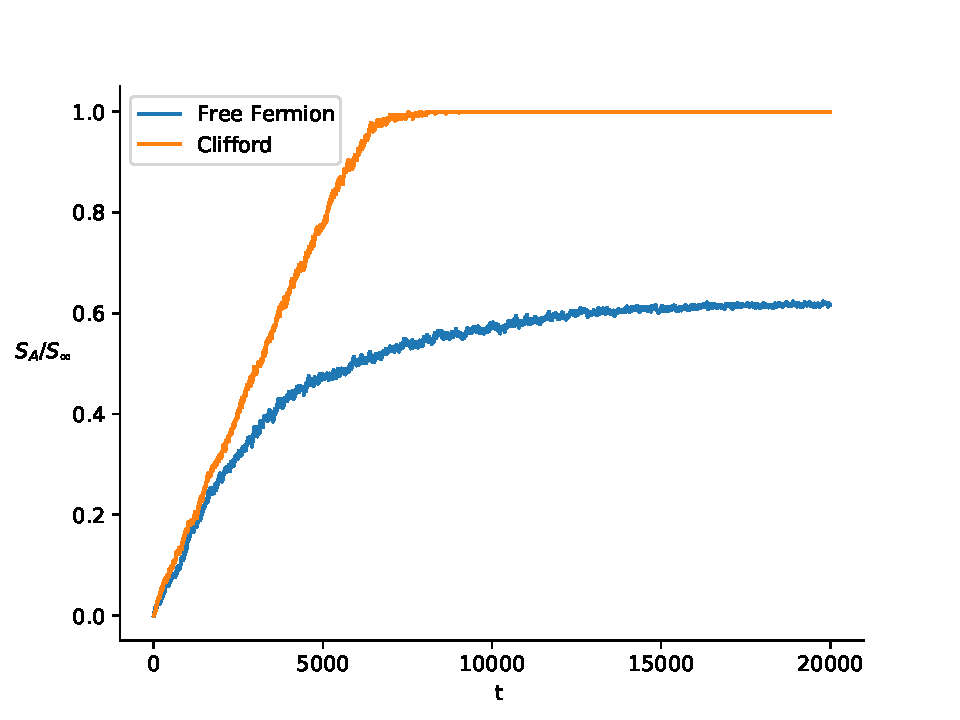
\includegraphics[width = \textwidth]{QS_Images/circuit_compare.pdf}
                    \caption{Numerical results for Clifford circuit and free fermion circuit. System size: $L=100$}
                \end{figure}
            \end{column}
        
            \begin{column}{0.5\textwidth}
                \begin{itemize}
                    \item Free Fermion weakly entangle compared to Clifford circuits.
                    \item Entropy saturation occurs later in free fermion circuit
                    \item Clifford circuits: Exhibit entanglement entropy growth but no operator spreading. 
                    \item Free Fermion circuits: Exhibit both entanglement entropy growth and operator spreading, but weaker.
                \end{itemize}
            \end{column}
        
            
        
        
        \end{columns}
                
            \end{frame}
            
    

    % Circuits described using fermionic operators. Qubits become local fermionic modes. Gates are expressed at fermionic operators. 
    % Anti-commutation relations - require a non-local description again, but can exhibit operator spreading in fermionic operators - reveals problems with the notion of locality. Fermions are inherently non-local, why?

    % Results, Show operator spreading for fermions, entanglement entropy for specific gates, what do the gates do? good image for this, 


\input{QS_Subfiles/QS_results.tex}

\begin{frame}{Further Directions}
    \begin{itemize}
        \item Changing geometry of free-fermion circuits to boost entanglement growth. 
        \item Finding new, less constrained sets of gates in the Clifford group to scramble operators.
        \item Recent work on dual-unitary circuits has shown them to be good candidates for the study of scrambling using tensor network methods. 
        \item Including higher-order terms in fermion circuits (interaction terms). 
    \end{itemize}
    
\end{frame}

\begin{frame}{Bibiliography}
    \bibliographystyle{ieeetr}
    \bibliography{QS_bibliography}
\end{frame}




%%%%%%%%%%%%%%%%%%%%%%%%%%%%%%%%%%%%%%%%%%%%%%%%%%%%%%%%%%%%
\end{document}

